% mn2esample.tex
%
% v2.1 released 22nd May 2002 (G. Hutton)
%
% The mnsample.tex file has been amended to highlight
% the proper use of LaTeX2e code with the class file
% and using natbib cross-referencing. These changes
% do not reflect the original paper by A. V. Raveendran.
%
% Previous versions of this sample document were
% compatible with the LaTeX 2.09 style file mn.sty
% v1.2 released 5th September 1994 (M. Reed)
% v1.1 released 18th July 1994
% v1.0 released 28th January 1994

\documentclass[useAMS,usenatbib]{mn2e}

% If your system does not have the AMS fonts version 2.0 installed, then
% remove the useAMS option.
%
% useAMS allows you to obtain upright Greek characters.
% e.g. \umu, \upi etc.  See the section on "Upright Greek characters" in
% this guide for further information.
%
% If you are using AMS 2.0 fonts, bold math letters/symbols are available
% at a larger range of sizes for NFSS release 1 and 2 (using \boldmath or
% preferably \bmath).
%
% The usenatbib command allows the use of Patrick Daly's natbib.sty for
% cross-referencing.
%
% If you wish to typeset the paper in Times font (if you do not have the
% PostScript Type 1 Computer Modern fonts you will need to do this to get
% smoother fonts in a PDF file) then uncomment the next line
% \usepackage{Times}

\usepackage{graphicx}
\usepackage{amsmath}
\usepackage{bm}
\usepackage{color}

%%%%% AUTHORS - PLACE YOUR OWN MACROS HERE %%%%%

%%%%%%%%%%%%%%%%%%%%%%%%%%%%%%%%%%%%%%%%%%%%%%%%

\title{Improving the removal of systematics in Kepler data}

\author[S. Aigrain et al.]{S. Aigrain$^{1}$\thanks{E-mail:
    suzanne.aigrain@astro.ox.ac.uk}, H. Parviainen$^{1}$,
  S. Roberts$^{2}$, S. Reece$^{2}$ \& 
  T.\ Evans$^{1}$ \\
  $^{1}$Sub-department of Astrophysics, Department of Physics,
  University of Oxford, Oxford OX1 3RH, UK\\
  $^{2}$Pattern Analysis and Machine Learining Group, Department of
  Engineering Science, University of Oxford, Oxford OX1 3PJ, UK}
\begin{document}

\date{Accepted \ldots Received \ldots; in original form \ldots}

\pagerange{\pageref{firstpage}--\pageref{lastpage}} \pubyear{2014}

\maketitle

\label{firstpage}

\begin{abstract}
TBD
\end{abstract}

\begin{keywords}
TBD
\end{keywords}

\section{Introduction}

During almost 5 years of operations, the Kepler space mission produced
continuous, high-precision light curves for over 150\,000 stars, with
a cadence of 29.4\,min. This forms a very rich dataset for a wide
range of stellar variability studies. However, the light curves also
contain instrumental artefacts and systematic trends. Correcting these while
preserving `real' astrophysical variability is challenging, but very
important for the community to make the most of the Kepler
data. 

The publicly available Kepler data products
\citep{KeplerArchiveManual} include three versions of the time-series
data for each target star. The target pixel files contain flux
measurements in each of the individual pixels falling within a
pre-defined area around each star. These have been corrected for known
instrumental effects at the pixel level, but are otherwise `raw'. The
light curve files contain two versions of the light curve, dubbed SAP
(simple aperture photometry) and PDC (pre-search data
conditioning). \citet{jen+10,KeplerDataProcHandbook} give an overview
of the data processing steps involved in producing both the target
pixel files and the light curves. The SAP light curves are obtained by
summing the flux falling within a subset of the pixels included in the
target pixel files, and applying a correction for background flux
\citep{twi+10a}. The PDC light curves result from additional
processing steps designed to remove instrumental artefacts and
systematics \citep{stu+12a,smi+12}.  As its name indicates, the PDC
pipeline is primarily intended to ready the data for planetary transit
searches, and is not specifically optimized to preserve other forms of
astrophysical variability.  The PDC data are nonetheless widely used
for variability studies \citep[for example stellar rotation studies,
see e.g.][]{rei+13,nie+13,mcq+13a,mcq+13b,mcq+14}, because they are
the only widely available set of light curves which cover the full
baseline of Kepler observations and are relatively free of the
systematics which dominate the SAP light curves. However, there are
also known problems: different versions of the PDC pipeline are, to
some degree, prone to over-correction (removal of real astrophysical
variability and injection of additional noise, see
e.g. \citealt{rob+13}). This motivated us to investigate alternative
methods to identify and correct systematic trends, with a specific
emphasis on retaining real astrophysical variability.

The Kepler detector consists of 21 modules arranged in a $5 \times 5$
grid with missing corners, each containing two
$4{\rm K}\times 2 {\rm K}$ CCDs \citep{KeplerInstHandbook}. The two
halves of each CCD are read out separately, leading to 4 output
channels per module. Throughout this paper, we refer to each module
plus output channel combination as a modout and identify it as $X.Y$
where $X$ is the module number (2 to 24) and $Y$ the output channel number (1 to
4). For the tests described in this paper, we focussed on 4 modules: 2.1, 7.3,
13.1 and 17.2. These were selected because they are collectively
representative of the range of systematic effects which affect Kepler
data: 2.1 is located near the upper left corner of the field of view
and is particularly sensitive to focus changes, 7.3 is `atypically
typical', 13.1 is at the centre of the focal plane, and 17.2 contains
some peculiar image artefacts (J.\ Smith, priv.\ comm.). 

Every three months, the Kepler satellite rolls by $90^{\circ}$ about its boresight
in order to keep its solar panels pointing towards the Sun. Each
3-month period between rolls is known as a quarter. As each star
falls on a different modout in each quarter, the systematics observed
vary from quarter to quarter, and their treatment is best
carried out separately for each quarter. Each star returns to
approximately the same position on the detector every 4 quarters (1
year), so the systematics observed in a given star's light curve in
quarters (say) 3 and 7 tend to be mutually similar. The systematics
are easier to correct in some quarters than in others: in this paper
we use quarter 3 (Q3) as an example of a relatively well behaved quarter,
and quarter 2 (Q2) as an example of a problematic quarter.

\subsection{Systematics removal in the PDC pipeline}
\label{sec:pdc}

\begin{figure*}
  \centering
  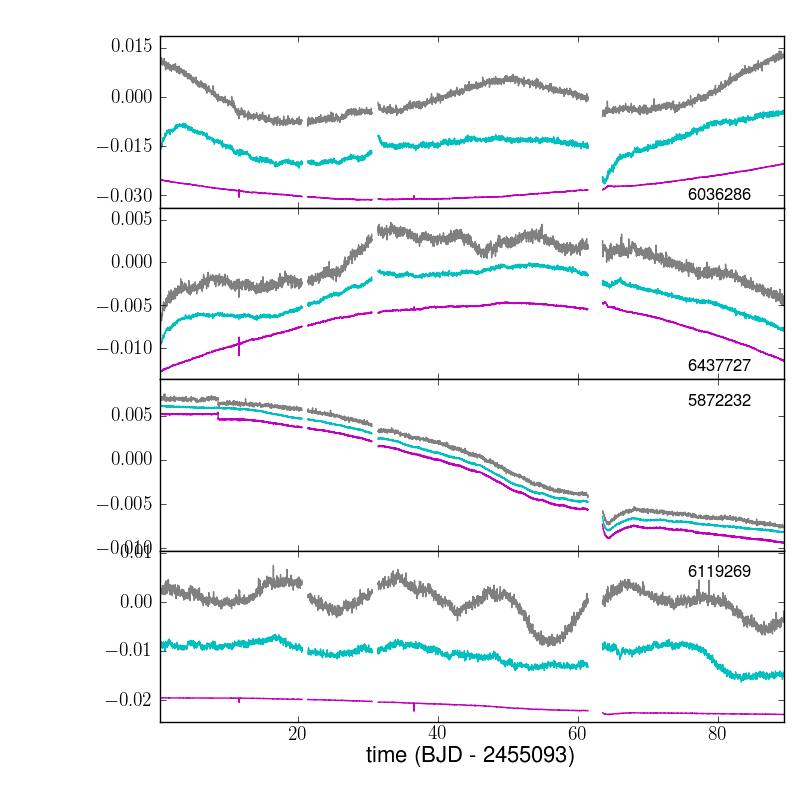
\includegraphics[width=0.49\linewidth]{fig1a.png} \hfill
  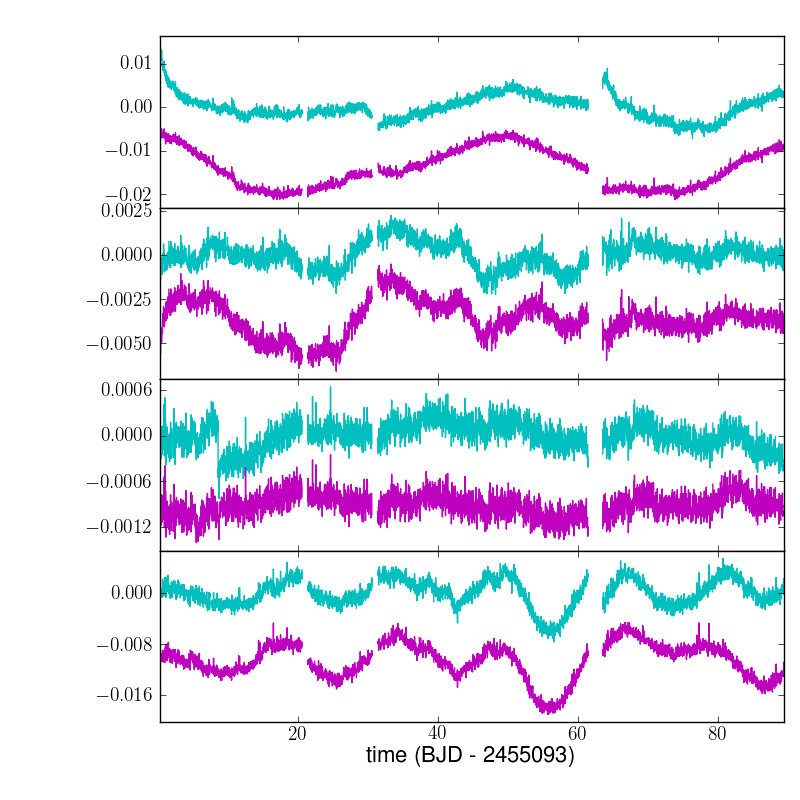
\includegraphics[width=0.49\linewidth]{fig1b.png}
  \caption{Example light curves before and after systematics
    correction (random selection from Q6, modout 7.3). The left column shows the SAP light curve for each
    object in grey, with the corrections applied by the PDC-MAP and
    by our own pipeline in cyan and magenta, respectively. The right column
    shows the corrected light curves (PDC-MAP in cyan, this work in
    magenta). In both columns, arbitrary vertical offsets have been applied
    to separate the different curves. The PDC-MAP correction is
    significantly more noisy than the CBV one, particularly in the top
    three cases. Note also the overcorrection of the intrinsic
    variability in the bottom case}
  \label{fig:ex_pdc}
\end{figure*}

In this subsection, we give a brief overview of the systematics
removal methods implemented in the pipeline which produces the
publicly available PDC light curves. This is a very simplified
description, intended only to set the scene for the present paper, and
a number of important features have been omitted for the sake of
brevity; full details are given in the relevant publications.

The standard approach for systematic trend removal in transit survey
data is to model each light curve as a linear combination of
systematic trends which are derived either from ancillary engineering
and meteorological data (such as telescope pointing, focus, seeing and
airmass, see e.g. \citealt{bak+07}) or from the light curves
themselves \citep{tam+05,kov+05}. In the latter case, variants of
Principal Component Analysis (PCA) are used to construct a reduced
basis from the light curves.

\begin{figure*}
  \centering
  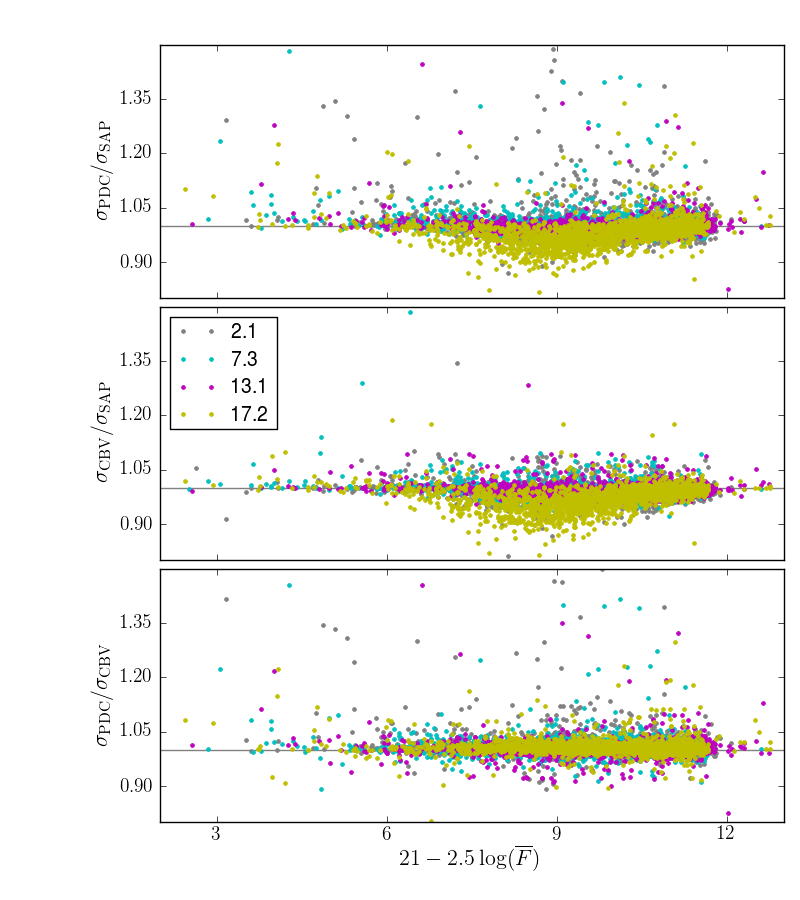
\includegraphics[width=0.49\linewidth]{fig2a.png} \hfill
  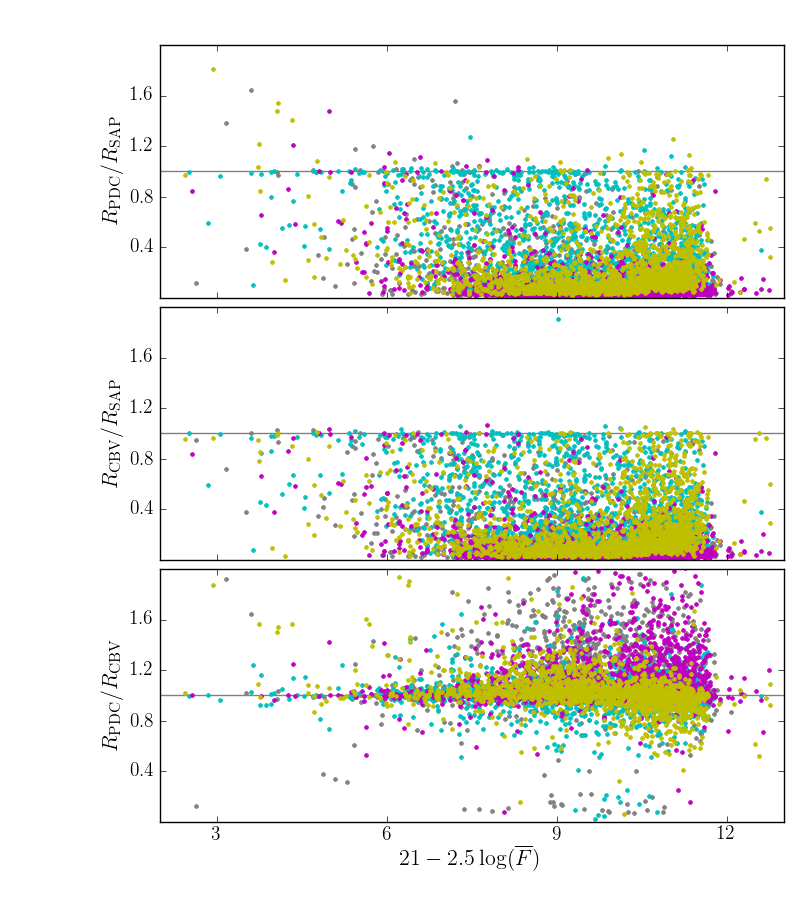
\includegraphics[width=0.49\linewidth]{fig2b.png}
  \caption{Statistical comparision of the SAP, PDC-MAP and CBV light
    curves for Q3. The left column shows the short-term scatter, $\sigma$ and
    the right hand column shows the range, $R$ (see text for
    definitions). In all cases, the x-axis shows a magnitude-like
    quantity based on the median flux in each light curve. The
    different colours correspond to different modouts (see legend in
    middle left panel). The detailed behaviour of the different modouts is discussed
  in Section~\ref{sec:comp}.}
  \label{fig:sig_ran_comp}
\end{figure*}

The PDC pipeline broadly follows this paradigm. In its original
version \citep{twi+10a,twi+10b}, known as PDC-LS (for least squares),
the basis was constructed from ancillary engineering data and the
coefficient realting each systematic trend (each term in the basis) to
each light curve were derived by least-squares (or maximum likelihood)
fitting. However, this method suffered from two problems: overfitting
(removal of real astrophysical variability) and injection of noise
into the light curves (a side-effect of overfitting combined with
noisy basis vectors). 

To address these issues, a new version of the PDC was introduced,
known as PDC-MAP (for maximum a posteriori, \citealt{smi+12}). In the
PDC-MAP, the systematic trends (which are known, in Kepler jargon, as
co-trending basis vectors, or CBVs), are computed from the light curves
themselves, by applying singular value decomposition (SVD) to the 50\%
of the light curves which show the strongest mutual correlation. This
is done separately for each of the 4 output channels in each of the 21
modules composing the Kepler detector. The
coefficients linking each CBV to each light curve are then evaluated
in a two-step process. First, preliminary estimates are computed using
the same least-squares method as in PDC-LS. The resulting coefficients
are used to construct prior distributions which are parametrised
according to stellar magnitude and position on the sky, and the final
coefficients are found by maximising the marginal likelihood for each
star, subject to these priors.

The PDC-MAP performs significantly better than the PDC-LS, and it is
less susceptible to overfitting and noise injection, althougth these
effects do remain apparent in some of the light
curves. Figure~\ref{fig:ex_pdc_bad} shows a few representative
examples where the PDC-MAP pipeline clearly introduces noise and/or
overcorrects astrophysical variability.  This is also illustrated in a
statistical manner in the top row of Figure~\ref{fig:sig_ran_comp},
which illustrates the change in the white noise level and light curve
amplitude before and after correction by the PDC-MAP pipeline. We
measure the white noise level $\sigma$ as the standard deviation of
the first difference of each light curve (throughout this paper, all
light curves are assumed to be normalised by dividing them by the
median flux value). Using the first difference ensures that any
long-term trends are taken out of the equation. The PDC-MAP leaves
$\sigma$ unchanged in most cases and can even reduces it in certain
modouts, but there is always a significant number of cases where
$\sigma_{\rm PDC} \gg \sigma_{\rm SAP}$, i.e. PDC-MAP has injected
significant amounts of noise into the light curve. 

We use the range $R$, first introduced by \citet{bas+10a,bas+10b}, to
describe the light curve amplitude. $R$ is defined as the interval
between the $5^{\rm th}$ and the $95^{\rm th}$ percentiles of the
normalised flux values. It captures variations on a wide range of
time-scales, including both systematics and intrinsic
variability. Most light curves are initially systematics-dominated, so
the PDC-MAP correction should -- and does -- reduce $R$ signifciantly
in most cases. However, the PDC-MAP correction \emph{increases} $R$
for a few bright stars in each modout (Figure~\ref{fig:sig_ran_comp},
top-right panel). This behaviour is not what would be expected if the
correction was actually removing systematics. 

In addition to the general issues already mentioned, some quarters remain
particularly problematic. [ illusrate this with a
plot of a full light curve, over Q0-Q17, showing bad quarters]

The most recent data releases employ yet another PDC version,
PDC-msMAP (for multi-scale MAP, \citealt{stu+12b}), where a
band-splitting process is used to separate long, medium and short-term
effects, which are treated in different ways. Long-term effects are
removed using least-squares (PDC-LS), which results in the
near-complete removal of all variability, whether systematic or real,
on timescales longer than 20 days. Medium-term effects are treated
using the PDC-MAP approach, and short-term effects are not removed at
all. The motivation for this is to minimise the disruption of transit
signals by the PDC pipeline, but the side effect is that PDC-msMAP
data are unsuitable for variability studies. On the other hand, the
PDC-MAP CBVs (without band-splitting) continue to be made available
together with the SAP and PDC-msMAP light curves.

\subsection{Alternative systematics removal methods}

[Flesh out this section later -- mention methods using the target pixel
files, and also the methods used in the KASC]. 

In \citet[][hereafter Paper I]{rob+13}, we presented a new method to
identify and correct common-mode systematics (trends present, to a
greater or lesser extent, in the majority of light curves), which we
called the ARC (Astrophysically Robust Correction) method, as it was
specifically designed to minimize the risk of removing or altering
astrophysical variability along with the instrumental
systematics. Like the PDC, the ARC is based on decomposing each light
curve into a linear superposition of systematic trends, plus a unique
vector representing intrinsic variability and random noise, and like
in PDC-MAP the systematic trends are identified from the light curves
themselves, for each output channel. The main differences are a) that
the ARC uses an information entropy criterion to identify and retain
only candidate trends that are genuinely systematic, i.e. composed of
small contributions from many light curves b) that the trends are
smoothed before they are corrected, to minimise the risk of
injecting noise into the corrected light curves, and c) that adaptive,
zero-mean (shrinkage) priors were used to evaluate coefficients
linking each systematic trend to each light curve. The ARC uses a
variational inference framework to carry out Bayesian inference under the linear basis
model (see the Appendix of paper I for full details), which is
extremely fast: once the basis vectors have been identified,
correcting all the light curves takes only 15 CPU minutes per quarter (SR TO CHECK).

The trend smoothing and the use of shrinkage priors mean that the ARC should be
even less prone to overfitting and noise injection than the PDC-MAP,
which is indeed what we found when comparing the two methods on
quarter 1 (Q1) data. However, before the ARC can be applied to later
quarters, the smoothing step must be revisited: in Paper 1, we used a
method called empirical mode decomposition (EMD, [ref]) to decompose
each trend into what are essentially distinct oscillatory modes with
different numbers of turning points, and retained only the mode with
the largest variance. Later quarters contain discontinuities and sharp
decays following each $\sim$ monthly data downlink event, which cannot
be captured adequately with EMD. We did investigate -- and are still
looking into -- alternative smoothing methods, in particular
modelling each trend with a Gaussian process (GP). If desired, the GP
model can be tuned to reflect any a priori knowledge on the
characteristics of the systematic effects which are expected to be
present (such as time-scale, quasi-periodic nature,
etc.). However, so far we did not converge on a completely
satisfactory trend-smoothing procedure.

On the other hand, we noted that the first few systematic trends
identified by the ARC (before de-noising) and the CBV tend to be
mutually quite similar, so that any differences in performance are
more likely to result from the trend smoothing and coefficient fitting
parts of the process than from the trend identification
process. Furthermore, both the first few ARC trends and the first few
PDC-MAP CBVs contain some high-frequency structure which appears to be
real, in the sense that it is also present in the light curves of
bright stars (where the photon noise does not mask these effects).
This is visible in the top left panel of Figure~\ref{fig:comp_sig_ran}
for modout 17.2 (yellow symbols). The PDC-MAP actually reduces the
white noise in most light curves, particularly those in the middle of
the magnitude range. In other words, not all of the short-term
variation in the CBVs is noise, which suggests that smoothing the
trends may not be optimal.

On the other hand, we have also seen that the PDC-MAP \emph{increases}
the white noise and appears to remove astrophysical
variability\footnote{This is a subjective statement, since we do not
  know which components of the variability in a given light curve are
  actually real, and which are systematic, but after visually
  examining many hundreds of Kepler light curves, one begins to build
  up a fairly robust prior on what kind of variations are systematic
  and what kind are not.} for a small but significant fraction of the
light curves. As we have shown in Paper 1, this problem is less
prominent for the ARC because of the use of adaptive, shrinkage
priors. This suggests a potentially `quick and easy' way to improve
the correction of systematic trends in Kepler data using existing
resources: by using the existing PDC-MAP CBVs, but the ARC shrinkage
prior approach. This is the subject of the present paper. 

An
additional motivation for developing an independent correction method
based on the PDC-MAP CBVs is that it enables us to quantify the effect of
the correction on stellar signals using injection tests (where
simulated signals are injected into the light curve before correction
and our ability to recover and characterise them after correction is
evaluated). We cannot do this for the PDC-MAP correction itself, as we
do not have access to the pipeline, only the data products.

\smallskip

The paper is structured as follows. In Section~\ref{sec:jumps} we
describe and test a method for identifying and correcting isolated
discontinuities in individual light curves. The correction of these
so-called sudden pixel sensitivity dropouts (SPSDs) is done as part of
the PDC, but the published data products do not provide enough
information to separate this from the systematic trend correction, so
it was necessary for us to develop our own SPSD correction. In
Section~\ref{sec:cbv} we describe our method for applying the PDC-MAP
CBVs to the light curves, which we call the CBV correction (to
distinguish it from the PDC-MAP correction). In particular we present a simple way of
deciding, for each light curve, how many CBVs should be used in the
correction. This Section also includes links to the corrected data and
the code used to produce them. In Section~\ref{sec:tests} we evaluate the performance of
our method using injection tests, and compare it to the PDC-MAP
method. [I may or may not add an additional section illustrating some
potential applications]. We discuss the potential applications of this
correctoin and summarise our conclusions in Section~\ref{sec:concl}.

\section{Detection and correction of individual discontinuities}
\label{sec:jumps}

The SPSD correction is roughly divided into three phases: the detection
of possible discontinuities, the identification of the found discontinuity 
candidates, and finally the correction of candidates identified as real
discontinuities.


% Step 1: Identification
% ----------------------
The SPSD candidate identification is carried out by first denoising the 
light curve in a way that aims to smooth the short time-scale scatter
while keeping discontinuities intact. We do this by modelling the flux 
as a Gaussian Process with an exponential kernel, and use the mean of the GP 
predictive distribution to represent the denoised light curve. Next, we
calculate the derivative of the light curve and identify the cadences where the
absolute slope deviates significantly from the slope distribution of the entire
denoised light curve as SPSD candidates. These steps are illustrated in 
Fig.~\ref{fig:jumps_identification}.


% Step 2: classification
% ----------------------
The Kepler light curves contain several types of signals that can cause rapid
changes in the flux. Besides the instrumental SPSDs that we want to find and correct, 
we also have astrophysical signals---such as planetary transits, binary eclipses, and stellar 
flares---that we do not want to remove. Thus, an automated SPSD correction routine
needs a way to identify an SPSD from these other discontinuities. We use a 
Bayesian information criterion (BIC)-based model selection approach for the
SPSD candidate classification. The method fits four different models to each SPSD candidate
(false alarm, transit-like, flare, or SPSD), modelling the flux baseline with a
Gaussian Process, and classifies the SPSD candidate based on the model BIC-values.

% Step 3: Correction
% ------------------
Finally, we correct the identified SPSDs based on the fitted discontinuity model and
save the information about the identified discontinuities for later use. The results
for an example light curve with several injected SPSD and transit signals are shown 
in Fig.~\ref{fig:jumps_classification}.

\begin{figure}
 \centering
 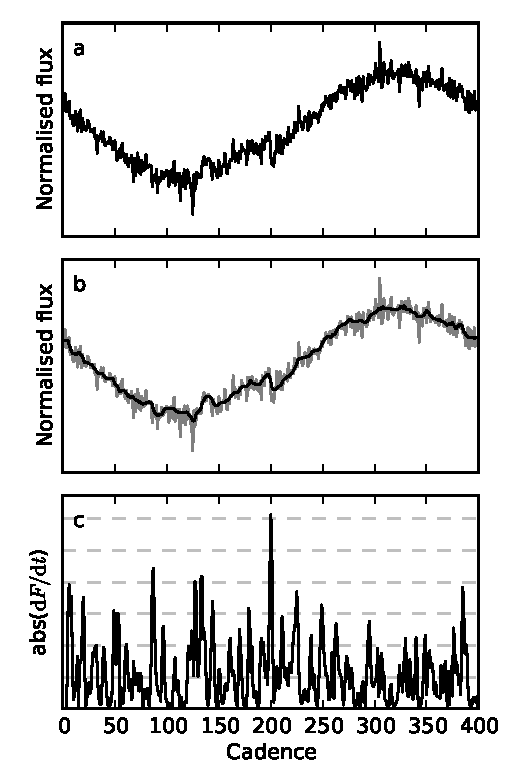
\includegraphics[width=\columnwidth]{jumps_identification.pdf}
 \caption{An example illustrating the basic steps for the SPSD candidate search: 
  and artificial light curve containing long-period variability, white noise,
  correlated noise, outliers, and an SPSD signal (a),
  the denoised light curve (b), and the absolute slopes of the denoised light
  curve (c) with the 1--6 standard deviations of the absolute slope distribution 
  marked as horizontal lines.}
 \label{fig:jumps_identification}
\end{figure}

\begin{figure*}
 \centering
 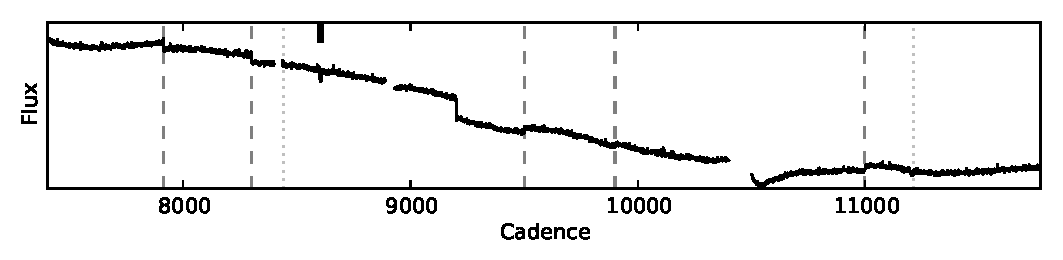
\includegraphics[width=\textwidth]{jumps_classification.pdf}
 \caption{The results of the SPSD search for a single light curve. The identified SPSDs
  are marked with dashed vertical lines, the identified transits as wide dashes, and the
  identified false-alarms as dotted lines. One transit-like feature has been mistakingly
  identified as false-alarm, and the search method has been told to ignore the single 
  high-amplitude SPSD.}
 \label{fig:jumps_classification}
\end{figure*}

\section{Optimized use of the CBVs}
\label{sec:cbv}

\subsection{CBV fitting using Variational Bayes}

We fit each light curve using the standard linear basis model:
\begin{equation}
F^{(i)}_j = \sum_{k=1}^K w^{(i)}_k C_{kj} + \epsilon^{(i)}_j
\end{equation}
where $F^{(i)}_j$ is the flux measured for star $i$ in observation
$j$, $C_{kj}$ is the value of the $k^{\rm th}$ basis vector
(systematic trend, or CBV) in observation $j$, $w^{(i)}_k$ is the
coefficient, or weight, relating basis vector $k$ to light curve $i$,
and $\epsilon^{(i)}_j$ represents the residuals of the correction for
star $i$ in observation $j$. In the remainder of this section, we omit
the superscript $^{(i)}$ for simplicity -- the analysis is done
separately for each light curve. Note that $\epsilon$ contains both
intrinsic variability and noise, representing the total residual for the
purposes of the systematics correction.

In a simple least-squares framework (such as PDC-LS), one seeks the
set of $w$'s which minimises the total squared residuals, $
\sum_j \epsilon_j^2 $. If the residuals are assumed to drawn
independently from a Gaussian distribution with known precision (inverse
variance) $\beta$ this is equivalent to
maximising the likelihood of the model:
\begin{equation}
p(\mathbf{F}|\mathbf{w},\mathbf{C}) =
\mathcal{N}(\boldsymbol{\epsilon};0,\beta^{-1} \mathbf{I}).
\end{equation}
(Note that strict equivalence only holds if $\beta$ is known, if it is
a free parameter then the full likelihood expression must be used.)

Maximum likelihood linear basis models are notoriously prone
to overfitting. Better results can be obtained in a Bayesian
framework, by using
priors over the $w$'s to encapsulate any external information
available over the expected values for the weights, and maximise the
posterior distribution instead of the likelihood. 
\begin{equation}
p(\mathbf{w}|\mathbf{F},\mathbf{C}) =
\frac{p(\mathbf{F}|\mathbf{w},\mathbf{C})  \, p(\mathbf{w})}{\int
  p(\mathbf{F}|\mathbf{w},\mathbf{C}) \, p(\mathbf{w}) \, {\rm d}\mathbf{w}},
\end{equation} 
where the normalisation constant in the denominator is the model
evidence $p(\mathbf{F}|\mathbf{C})$. In the PDC-MAP, the priors over
the $w$'s are based on the distribution of the coefficients derived in
the maximum likelihood case (i.e.\ in the absence of priors),
parametrised as a function of star position and magnitude. This
reflects the belief that stars which are near each other on the
detector and have similar brightnesses should also display similar
systematics. As we have seen, it does reduce the overfitting problems
which had been noted in PDC-LS, but does not entirely do away with
them. One plausible explanation for this is that the PDC-MAP priors
themselves are affected by overfitting in the initial, maximum
likelihood step. Furthermore, a fixed prior, as in the MAP model,
does not guarantee model shrinkage as required to avoid overfitting. 

To reduce the risk of overfitting further, we propose to use priors
which specifically penalise larger weights, and make it less likely
that one basis vector will compensate for another. A natural choice
for this is to use zero-mean Gaussian priors:
\begin{equation}
p(w_j|\alpha_j) = \frac{\alpha_j}{\sqrt{2 \pi}} \exp\left(-\alpha_j w_j^2 / 2 \right)
\end{equation}
for each $j$ (the individual prior weights are treated as
mutually independent).  Furthermore, we do not fix the priors, but
instead treat the inverse variances, $\boldsymbol{\alpha}$, as
parameters themselves, subject to their own prior
$p(\boldsymbol{\alpha})$, for which we use a Gamma
distribution\footnote{Our choice of priors over $\mathbf{w}$ and
  $\boldsymbol{\alpha}$ is also mathematically convenient, because
  they are conjugate with each other and with the likelihood (which is
  Gaussian), enabling a number of the integrals involved in the
  inference to be performed analytically.}. Unless there is strong evidence for a non-zero weight
for particular light curve / basis vector combination, the Gamma prior over
$\alpha$ will tend to make the prior over $w$ collapse to a delta
function centred on zero, so most basis vectors will have zero weight in most
light curves. This is sometimes referred as
automatic relevance determination (ARD) or shrinkage.

We then seek to evaluate the posterior distribution over the weights
$\mathbf{w}$, marginalised over the prior precisions
$\boldsymbol{\alpha}$:
\begin{equation}
p(\mathbf{w}|\mathbf{F},\mathbf{C}) \propto \int
p(\mathbf{F}|\mathbf{w},\mathbf{C})  \, p(\mathbf{w}|\boldsymbol{\alpha}) \, p(\boldsymbol{\alpha}) \, {\rm d}\boldsymbol{\alpha},
\end{equation} 
and to maximise it with respect to $\mathbf{w}$. In general, the
posterior distribution is unknown and is not analytically
tractable. Numerically evaluating and optimizing the posterior would
require evaluating the likelihood over a very large number
of $(\mathbf{w},\boldsymbol{\alpha})$ combinations, which is
unfeasible, especially as it needs to be done for every Kepler
light curve. 

An elegant workaround consists in approximating the posterior with a
proposal distribution which is analytically tractable, and iteratively
refining the latter so that it approaches the true posterior. This
class of methods is known as approximate inference. More specifically,
one can restrict oneself to proposal distributions which belong to the
exponential family: refining the proposal then consists in optimising
an integral with respect to a functional, which is typically done
using the calculus of variations. This approach is thus known as
variational inference, or variational Bayes (VB). A detailed
description of the VB method as applied to our linear basis model was
given in the appendix of Paper I, so we do not repeat it here. The
algorithm essentially consists in cycling through a set of update
equations for the weights $\mathbf{w}$, the prior precisions
$\boldsymbol{\alpha}$ and the noise precision $\beta$. Importantly,
the model is guaranteed to improve each iteration, thus providing robust
convergence which typically occurs after just a few 
iterations. The computational requirement scales as $JK^2$, where $J$
is the number of observations and $K$ is the number of basis
vectors. Our {\sc Matlab} batch implementation of the method runs in
$< 3$ minutes (on a quad-core i7 CPU) per output channel ($1500$--$2000$
stars) and per quarter ($\sim 4300$ observations) for up to 8 CBVs. 

\subsection{How many CBVs?}

\begin{figure*}
  \centering
  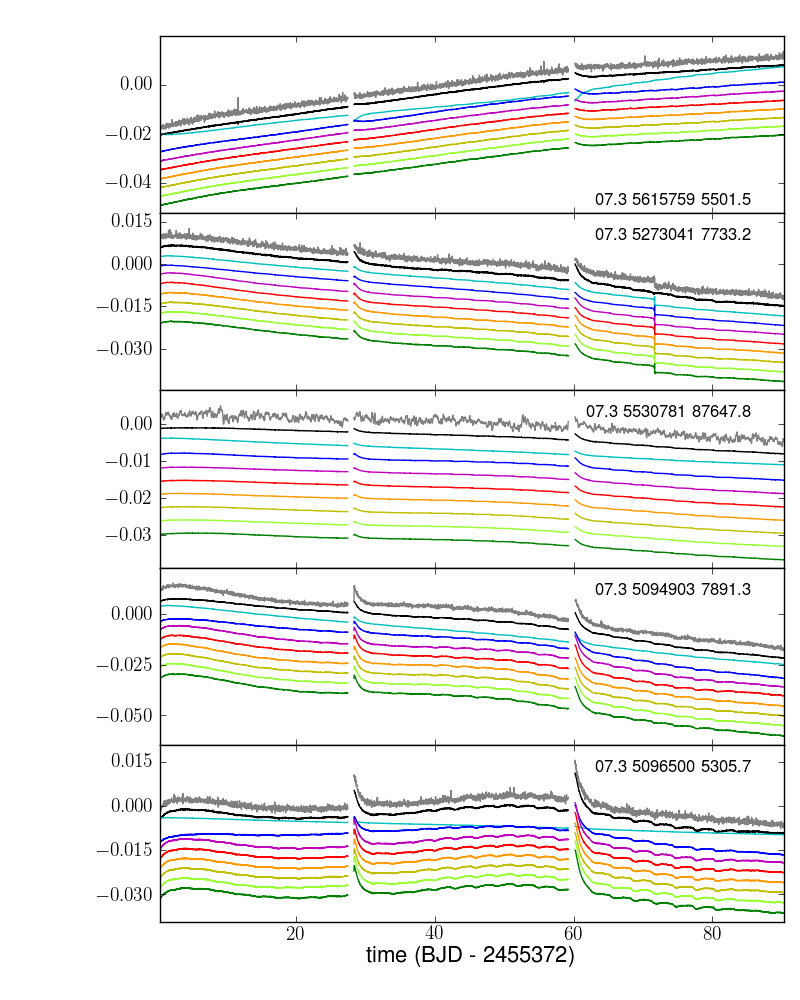
\includegraphics[width=0.49\linewidth]{q6_mod07_out3_cbv_examples_diff.png}
  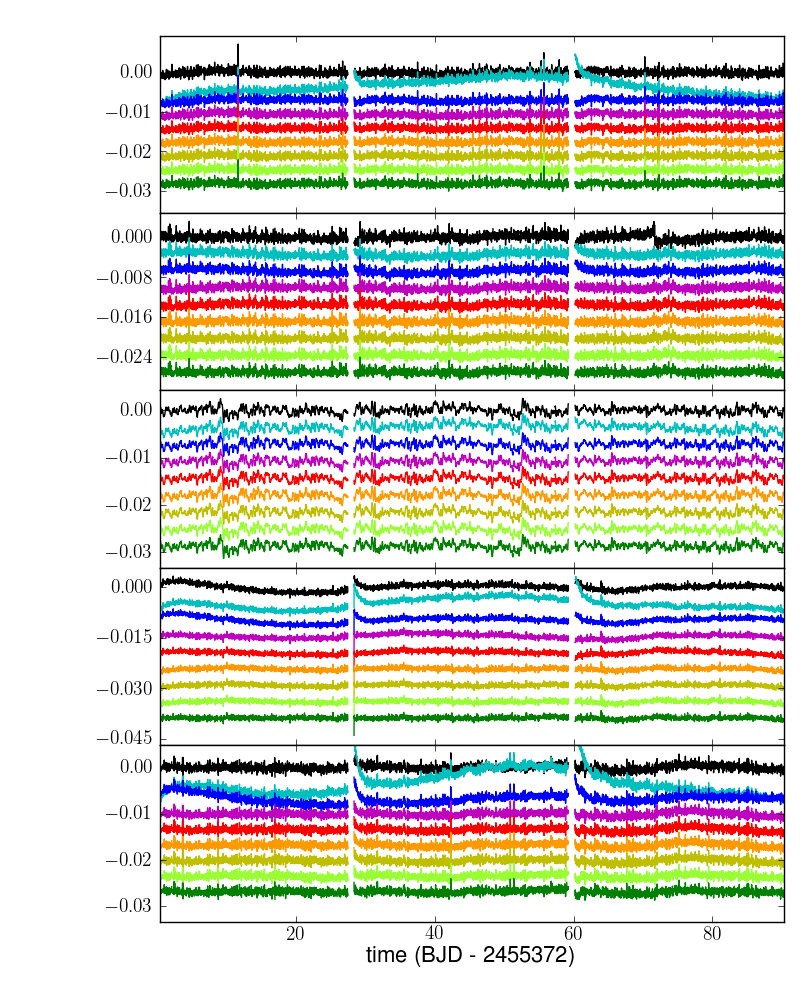
\includegraphics[width=0.49\linewidth]{q6_mod07_out3_cbv_examples.png}
  \caption{Comparison of the systematics correction using 1 to 8 CBVs,
    for a random selection of stars in Q3, modout 17.3. The left panel
    shows the original (SAP) light curve in grey and the corrections
    applied using 1 to 8 CBVs in different colours (cyan to green, and
    top to bottom). The PDC-MAP correction is also shown in black, for
    comparison. The right panel shows the corrected light curves,
    using the same colour-coding. In both panels, the different light
    curve versions have been offset by an arbitrary amount, for
    clarity. [Will find better, more illustrative examples when I get
    the chance]}
  \label{fig:ncbv_ex}
\end{figure*}

Despite the measures described in the previous section to minimise the
risk of overfitting, the results still depend, in some cases, on the number of basis vectors
used. The PDC-MAP CBVs result from a singular value decomposition of a
subset of the light curves, and therefore the first CBV represents a
larger fraction of the overall variance of the light curves, and so
on... The PDC-MAP pipeline saves 16 CBVs but only uses at most 8 to
perform the correction. Additionally, a signal-to-noise ratio (SNR)
criterion is used to exclude CBVs which are deemed to contribute more
noise than useful information (see \citealt{smi+12} for details), so
the actual number of CBVs used ranges from 5 to 8. 

As the VB method is very fast, it is feasible to run it for every possible
number of CBVs, $K$ (from 1 to 16). We first did this for a few
representative quarters (3 to 6) and output
channels, and performed a visual comparison of the results on a random
selection of light curves. 

We plotted the original (SAP) light curve, the correction
applied and the corrected light curve, for a few tens of stars
selected at random in each modout. A few examples are shown in
Figure~\ref{fig:ncbv_ex}. In most cases, the overall
shape of the correction is fairly insensitive to the number of CBVs
used, so long as it is at least than 2 or 3. On the other hand, as the
CBVs are increasingly noisy, using more CBVs introduces more noise
into the light curves particularly for the brighter stars. It is
therefore important to use the smallest number of CBVs which gives an
adequate correction. Importantly, the examples we examined 
suggest that this number differs from star to star: in some cases,
including the $4^{\rm th}$ and $5^{\rm th}$ CBVs removes features
which appear systematic in nature, and which were not removed when
using only the first two. In other cases, even using the $2^{\rm nd}$ CBV
appears to have a detrimental effect.

Rather than specifying an overall value for $K$ for, say, each
quarter and modout, we therefore decided to select the optimal number
of CBVs to use \textit{a posteriori}, on a light curve by light curve basis,
based on a statistical comparison of the light curve properties before
and after correction, using the simple statistics $R$ and $\sigma$. 

If most light curves are
initially dominated by systematics, the dependence of $R$ on $K$
tracks the extent to which the correction of systematics is improved
by adding more CBVs. Typically, $R$ decreases rapidly for low $K$ but
then reaches a plateau for larger $K$. Within this plateau regime, increasing
$K$ beyond does not usually improve the correction
significantly but it does introduce more noise, so one might simply
opt for the lowest value of $R$ at which the plateau is
reached. We initially define $K_{\rm opt}$ as the smallest value of $K$ for which $R(K)
< \langle R \rangle + 3 \sigma_R$, where $\langle R \rangle$ and
$\sigma_R$ are the median and standard deviation of $R$ over all
values of $K$, for a given light curve. 

However, when the initial amplitude of systematics is small relative
to that of the intrinsic variability, this criterion alone is
insufficient: $R$ can decrease with increasing $K$ not because more
systematics are being removed, but because real variations are
actually being removed. This particularly frequent for bright,
variable stars. One way of testing for this would be to inject
realistic simulated variability signals into the light curve before
correction, and check how well they are recovered
post-correction. However, doing this for every light curve would be
prohibitively expensive. We do use such injection tests can be used to
evaluate the overall ability of our correction method to preserve
astrophysical signals, but only on a subset of the data (see
Section~\ref{sec:inject}).

Fortunately, there is an easier way to
identify these problematic cases: visual inspection shows that, when
the correction removes what looks like real variability, it also
introduces significant amounts of high frequency noise into the light curves. This can be
diagnosed by tracking the dependence of $\sigma$ on $K$. Specifically, if
$\sigma(K_{\rm opt})/\sigma_0>1.1 $, where $K_{\rm opt}$ is determined
from the behaviour of $R$ as described above, and $\sigma_0$ is the
short-term scatter before correction, $K_{\rm opt}$ is decreased further
until the scatter ratio falls below the 1.1 threshold. The choice of
threshold is somewhat arbitrary, but its exact value is not
critical: when it is exceeded it is usually by a fairly wide margin.

[include a figure illustrating the selection of $K_{\rm opt}$ for a
straight-forward case, and one where the $\sigma$ threshold had to be
used.]

Having defined a method for selecting $K_{\rm opt}$, we processed
all the Kepler data publicly available at the time of writing,
i.e. quarters 0 to 17. The resulting corrected light curves are
publicly available at [include URL], along with the code used to
produce them. There are two versions of the code: a batch version,
written in {\sc Matlab}, which processes entire modouts, and a
single-light curve version, written in {\sc Python}, which works
directly on the FITS light curve and CBV files produced by the Kepler
pipeline. In the next Section, we test the performance of the CBV
correction using injection tests, and compare it to the PDC-MAP
results.

\section{Performance tests}
\label{sec:tests}

\subsection{Injection tests}
\label{sec:inject}

\begin{figure*}
  \centering
  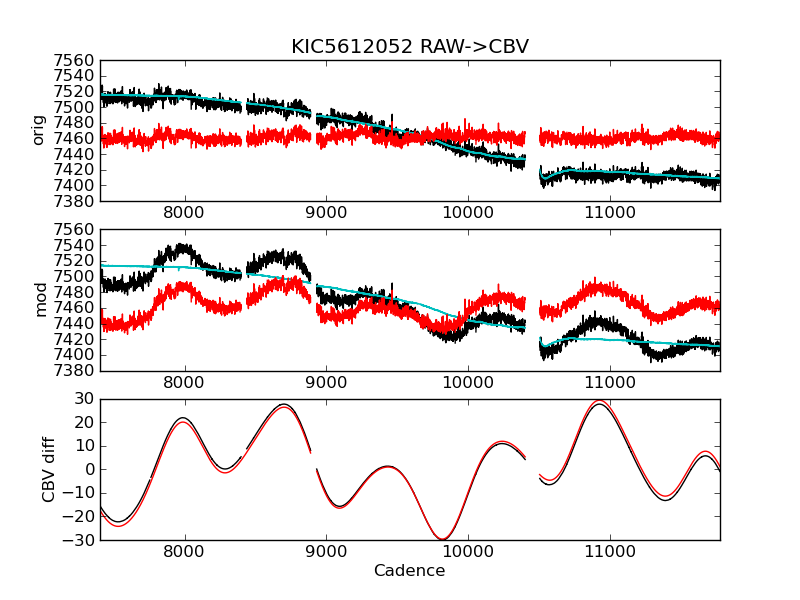
\includegraphics[width=0.48\linewidth]{inject_ex1.png} \hfill
  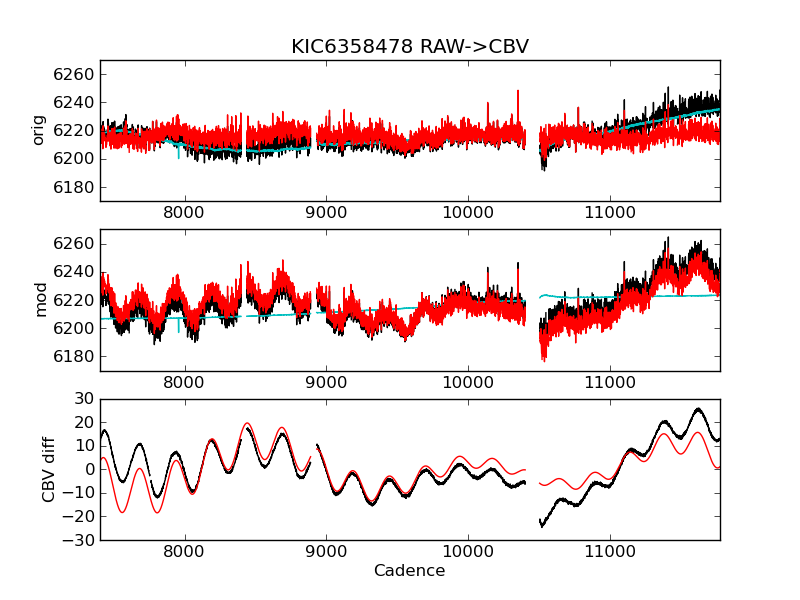
\includegraphics[width=0.48\linewidth]{inject_ex2.png}
  \caption{Injection test examples (Q3, modout 17.2). Top: original
    and corrected light curve (black and red, respectively) with the correction
    shown in cyan. Middle: same after injecting the simulated
    signal. Bottom: injected and recovered signals (red and black, respectively.}
  \label{fig:inject_ex}
\end{figure*}

The method we use to select the number of CBVs used, as described in
the previous Section, is intended to remove systematics as effectively
as possible while minimizing the risk of
overfitting, i.e. removing astrophyiscal variability, and of
introducing extra noise into the light curves due to the noisy nature
of the CBVs themselves. To test the extent to which our systematics
removal method affects stellar variabiltiy, we now perform a series of
injection tests. Specifically, we are interested in variability caused
by rotational modulation of surface inhomogeneities such as
star-spots, since this is a powerful diagnostic of stellar rotation
rates and hence angular momentum evolution.

\begin{figure*}
  \centering
  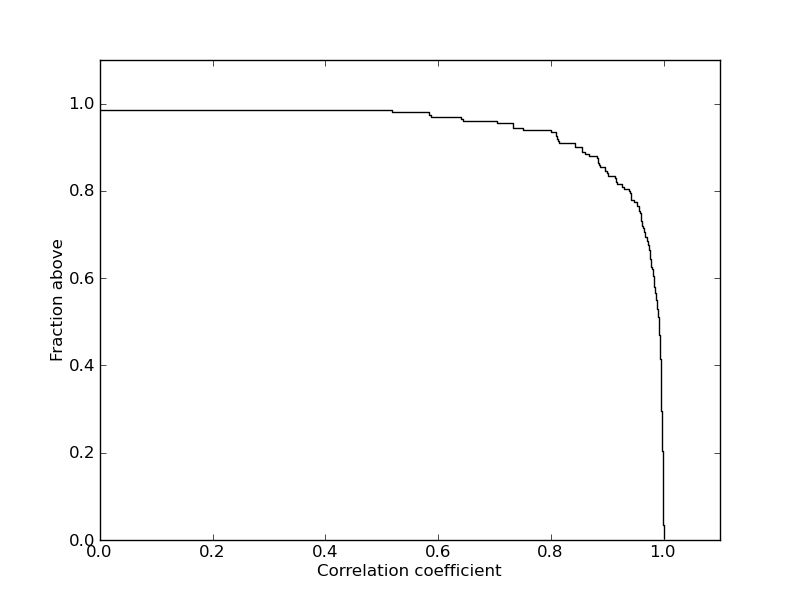
\includegraphics[width=0.245\linewidth]{inject_stat_corr_coeffs.png} \hfill
  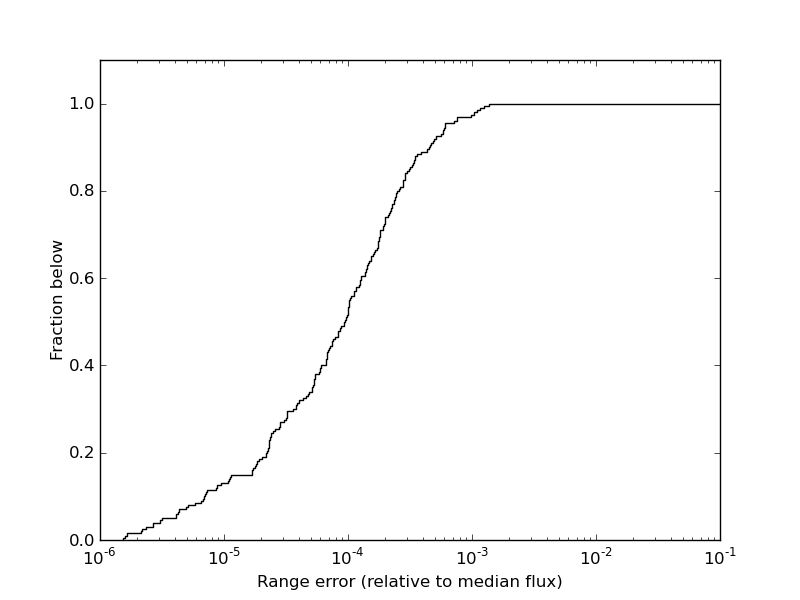
\includegraphics[width=0.245\linewidth]{inject_stat_ranges.png} \hfill
  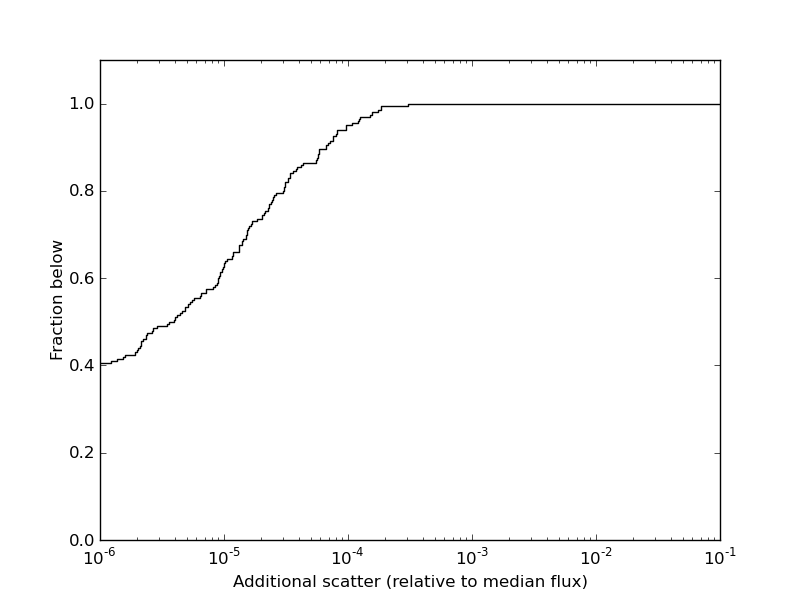
\includegraphics[width=0.245\linewidth]{inject_stat_scatt.png} \hfill
  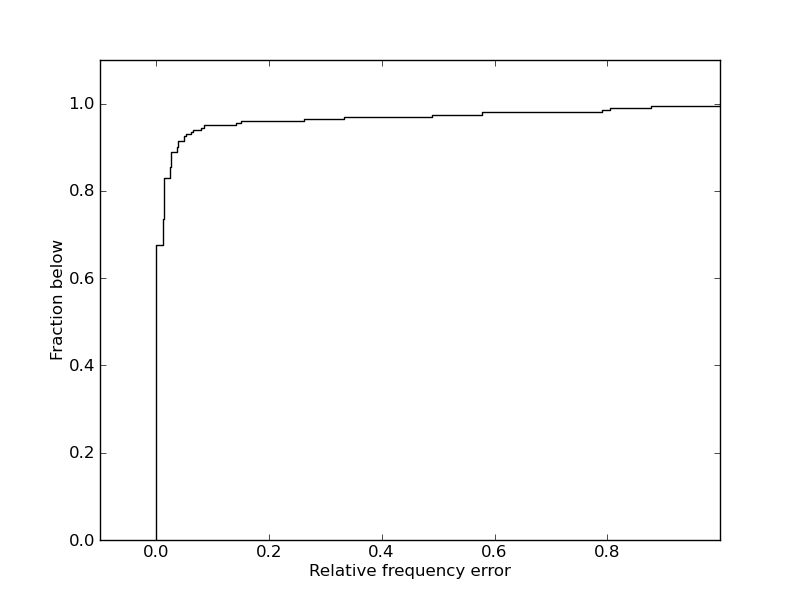
\includegraphics[width=0.245\linewidth]{inject_stat_freqs.png} 
  \caption{Cumulative distributions of the Pearson correlation coefficient between
    injected and simulated signals (left), the range error (difference
    between ranges of injected and recovered signal, middle left), the scatter
    injected by the correction (scatter of recovered signal minus
    scatter of injected signal, middle right) and the relative
    frequency error (difference between the measured frequencies in
    the injected and recovered signals, divided by the former, right).}
  \label{fig:inject_stat}
\end{figure*}

We simulate rotation-like signals, consisting of between 1 and 5 co-added
sinusoidal variations, with periods randomly drawn from a log uniform
distribution ranging from 5 to 60 days, and amplitudes drawn from a
log normal distribution with mean $10^{-3}$ and standard deviation 0.5
dex. These were added to 200 randomly select light curves in each
modout, which were then corrected for systematics as described in the
previous section. The difference between the corrected light curves
with and without injected signal, hereafter referred to as the
\emph{recovered} signal, is then compared to the injected
signal itself: any discrepancies arise because the correction is affecting
the injected signal. Figure~\ref{inject:ex} illustrates this process
for a few example light curves. Of course, the light curves into which the
simulated signals are injected already contain astrophysical
variability, which themselves may have been affected by the
correction, and this may contribute to the differences between the
injected and recovered signals. However, we opted for this approach
rather than attempting to generate light curves with simulated stellar
signals \emph{and} systematics, because we do not have a good
generative model for the latter. 

We quantify the effect of the correction on the simulated signals by
measuring the Pearson correlation coefficient $P$ between the injected
and recovered signal, and by comparing the range $R$, scatter $\sigma$
(as defined earlier) and frequency $F$ of the injected and recovered
signals. The results are shown for a representative modout in
Figure~\ref{inject:stat}. $F$ was measured by simple least squares
fitting of a sinusoid over a grid of equally spaced trial
frequencies. These plots show that the injected signals are remarkably
well preserved: $P$ is $>0.9$ and the error in $R$ is $<500$\,ppm 83\%
of the time, white the added scatter is $<100$\,ppm and the relative
frequency error $<0.05$ 92\% of the time. These plots shown are for
modout 17.2 in Q3, but the same tests were performed for all 4 of the
test modouts in Q3--Q6 inclusive, and gave similar results. We also
checked for any correlation between the metrics discussed above and the
amplitude or frequencies of the injected signal compared to the range,
scatter and frequency of the original light curve after correction,
but did not find any significant trends.

\subsection{Comparison to PDC-MAP}
\label{sec:comp}

Figures~\ref{fig:ex_pdc} and \ref{fig:sig_ran_comp} show a comparison
of the PDC-MAP and CBV corrections using illustrative examples and
quantitative statistics, respectively. The most important feature, in
both cases, is that the corrected light curves and associated
statistics are generally similar. This is not altogether surprising,
since both corrections are based on the same set of basis vectors, but
it is reassuring: it indicates that the different choices of priors do
not usually have too strong an effect on the results. Nonetheless, for
a subset of the cases, the PDC-MAP correction is significantly more
noisy than the CBV one, as illustrated by the left panel panel of
Figure~\ref{fig:ex_pdc} (particularly rows 1, 2 and 4) and the bottom
left panel of Figure~\ref{fig:sig_ran_comp}. The number of cases where
the scatter is significantly increased after correction is also
significantly lower in the CBV case than in the PDC-MAP one. In
quantitative terms, the median value of $\sigma_{\rm PDC}/\sigma_{\rm
  CBV}$ was 1.004 for the 4 modouts considered in Q3, but the number of
cases where $\sigma_{\rm PDC}>1.1 \sigma_{\rm CBV}$ was 115 (out of
7935), whereas the number of cases where $\sigma_{\rm PDC}<0.9
\sigma_{\rm CBV}$ was only 19.

As an aside, we note that comparing $\sigma$ before and after
correction can be used as a useful diagnostic of problematic light
curves: when the CBV correction increases $\sigma$ by
more than 10\%, visual examination of the light curves often reveals
abnormal behaviour, apparently associated with image artefacts, stars
located near the edge of a CCD, or very high proper motion stars
(where the fraction of the flux collected within the photometric
aperture might change signficiantly during a quarter). [Need to
include a figure illustrating some of these]. We therefore flag these
light curves so that they can be identified readily. 

We now examine the behaviour of the range parameter $R$ (right
hand-panel of Figure~\ref{fig:sig_ran_comp}). The CBV correction
never increases $R$. This is so by design: the only circumstance in
which removing systematics should increase $R$ is one where the
systematics had somehow `conspired' to `cancel out' some of the real
variability, which is unlikely. Aside from that, the before and after
range comparison looks similar for the CBV and the PDC-MAP
correction. Direct comparison between the two shows broad similarity
(the median value of $R_{\rm PDC}/R_{\rm CBV}$ is 1.020 for the 4
modouts considered in Q3) but with significant modout-to-modout
differences.

[Include discussion of individual modout behaviour]



\section{Discussion and conclusions}
\label{sec:concl}

\bsp

\label{lastpage}

\bibliography{arc2}
\bibliographystyle{mn2e}

\end{document}
